\documentclass[final,3p,times]{elsarticle}

\usepackage{amssymb}
\usepackage{url}
\usepackage{hyperref}

\journal{SoftwareX}

\begin{document}

\begin{frontmatter}

\title{dynaRchetypes: An S4-based R engine for the unsupervised extraction of physical fault archetypes in continuous telemetry}

\author[1]{Jo\"{e}l R. Pradines\corref{cor1}}
\ead{joel.pradines@example.com} % Update with actual email
\address[1]{[Insert Affiliation/Institution Here]}
\cortext[cor1]{Corresponding author.}

\begin{abstract}
The proliferation of Cyber-Physical Systems (CPS) generates continuous multivariate telemetry that demands robust, interpretable diagnostic frameworks. Naive unsupervised anomaly detection frequently fails in these environments, as static spatial clustering of raw telemetry ignores temporal history and fragments operational states into diagnostic noise. We introduce \textit{dynaRchetypes}, an open-source R package that bridges mathematical anomaly isolation with deterministic physical routing. The software pairs an Isolation Forest engine with Multivariate Dynamic Time Warping (MDTW) to extract structural breaks and group them into cohesive physical fault archetypes. In this paper, we demonstrate that kinematic feature engineering (temporal derivatives) is strictly required to preserve thermodynamic context within tree-based algorithms, outperforming Euclidean spatial clustering in preserving trajectory dynamics. The package introduces Explainable AI (XAI) ablation modules to physically interpret fault drivers, alongside automated reproducibility frameworks for hyperparameters. Finally, contiguous out-of-sample prognostic testing validates the architecture's capacity to prevent alert storms and maintain a stable triage queue during seasonal concept drift, providing a complete, human-in-the-loop diagnostic pipeline for operations research.
\end{abstract}

\begin{keyword}
Anomaly Detection \sep Multivariate Dynamic Time Warping \sep Explainable AI \sep Concept Drift \sep Cyber-Physical Systems
\end{keyword}

\end{frontmatter}

\section*{Current code version}
\begin{table}[!h]
\begin{tabular}{|l|p{6.5cm}|p{6.5cm}|}
\hline
\textbf{Nr.} & \textbf{Code metadata description} & \textbf{Please fill in this column} \\
\hline
C1 & Current code version & v0.1.0 \\
\hline
C2 & Permanent link to code/repository used for this code version & \url{https://github.com/JoelRMath/dynaRchetypes} \\
\hline
C3 & Code Ocean compute capsule & N/A \\
\hline
C4 & Legal Code License & MIT License \\
\hline
C5 & Code versioning system used & git \\
\hline
C6 & Software code languages, tools, and services used & R, YAML, C++ (via isotree) \\
\hline
C7 & Compilation requirements, operating environments & R ($\ge$ 4.1.0) \\
\hline
C8 & If available, link to developer documentation & \url{https://github.com/JoelRMath/dynaRchetypes/vignettes} \\
\hline
C9 & Support email for questions & [Insert Email] \\
\hline
\end{tabular}
\end{table}

\section{Motivation and Significance}

The proliferation of Internet of Things (IoT) sensors across Cyber-Physical Systems (CPS)—ranging from industrial robotics to HVAC infrastructure—generates unprecedented volumes of continuous multivariate telemetry \cite{cook2019anomaly}. Extracting actionable maintenance states from these noisy time-series streams is a high-value challenge in operations research.

Current anomaly detection methodologies generally fall into two main categories. Static, rule-based thresholds are computationally efficient and transparent, yet they struggle to capture kinematic fault trajectories and often yield elevated false-positive rates caused by seasonal drift. Conversely, Artificial Neural Networks (ANNs) offer robust multidimensional detection but act as "black boxes," meaning their internal decision-making processes are hidden from the operator \cite{blazquez2021review}. This lack of interpretability complicates human-in-the-loop triage; while an ANN may accurately flag a mathematical deviation, translating that anomaly into an actionable physical maintenance state remains a challenge.

To bridge the gap between static rules and black-box fault-detection models, we introduce \texttt{dynaRchetypes}, an open-source, S4-based R package designed to automate the extraction of physical fault archetypes. Built as a domain-agnostic engine, the software utilizes a YAML configuration schema to ingest user-defined features, keeping domain-specific logic separate from the core mathematical pipeline. Methodologically, it combines the generation of an Isolation Forest for fault extraction \cite{liu2008isolation} with Multivariate Dynamic Time Warping (MDTW) distances \cite{shokoohi2017generalizing} to group anomalies by their temporal trajectory rather than static spatial proximity. By extracting the geometric medoid of each cluster, the software isolates a representative temporal window, enabling direct visualization and interpretation of the specific fault type. Furthermore, algorithmic ablation provides explicit feature attribution to identify the sensors driving each fault.

\section{Software Description}

\texttt{dynaRchetypes} utilizes an object-oriented framework to manage the mathematical progression from feature extraction to temporal clustering.

\subsection{Decoupled Architecture}

A YAML configuration file allows the user to define both the domain-specific feature schema (e.g., \texttt{context\_variables} and \texttt{target\_variables}) and the machine learning hyperparameters (e.g., \texttt{anomaly\_threshold}, \texttt{temporal\_window\_hours}, and \texttt{ntrees}). Internally, the engine tracks its progression through lifecycle states (such as \texttt{telemetry\_ingested} and \texttt{calibrated}) to ensure the diagnostic pipeline executes in the correct sequence, preventing the user from calling downstream steps—such as clustering—before the model is calibrated.

\subsection{Software Functionalities}
The pipeline is executed through six primary methods:
\begin{enumerate}
\item \textbf{\texttt{ingest\_telemetry()}:} Parses the YAML schema, validates incoming datasets, and locks the computational feature matrix.
\item \textbf{\texttt{extract\_anomalies()}:} Calls a C++ backed Isolation Forest to evaluate the time-series data and identify time points with high anomaly scores.
\item \textbf{\texttt{compute\_distances()}:} Extracts a multivariate time-series window (e.g., $\pm 2$ hours) around each anomaly and computes a symmetric MDTW distance matrix.
\item \textbf{\texttt{calibrate()}:} Uses the MDTW matrix to build a Divisive Analysis (DIANA) tree. It then evaluates different cluster counts ($k$) to determine the optimal number of fault groupings, using metrics designed to prevent the formation of overly small, fragmented clusters.
\item \textbf{\texttt{commit\_queues()}:} Assigns anomalies to the optimal clusters identified during calibration and extracts the geometric medoid to provide the most representative variable dynamics of each cluster for plotting.
\item \textbf{\texttt{explain\_anomaly()}:} Calculates Z-scores and algorithmic ablation drops, allowing the user to rank sensors for their contribution to an anomaly.
\end{enumerate}


\section{Feature Selection and the Case for Isolation Forests}

To provide practical examples of usage and outline a standard workflow, we applied the \texttt{DiagnosticEngine} to a multi-year HVAC telemetry dataset (Turin, Italy) containing 31,000 continuous 15-minute intervals \cite{borda2022development}.

When selecting features for anomaly detection, managing correlated variables is critical. Feeding highly correlated data into general anomaly detection models—particularly distance-based algorithms—can distort feature weights and obscure genuine faults. Therefore, a standard initial step is to examine the linear correlation between variables. As illustrated in the correlation heatmap (Figure \ref{fig:correlation}), the Turin dataset exhibits numerous interdependencies, with several pairs of variables demonstrating high linear correlation.

\begin{figure}[htbp]
    \centering
    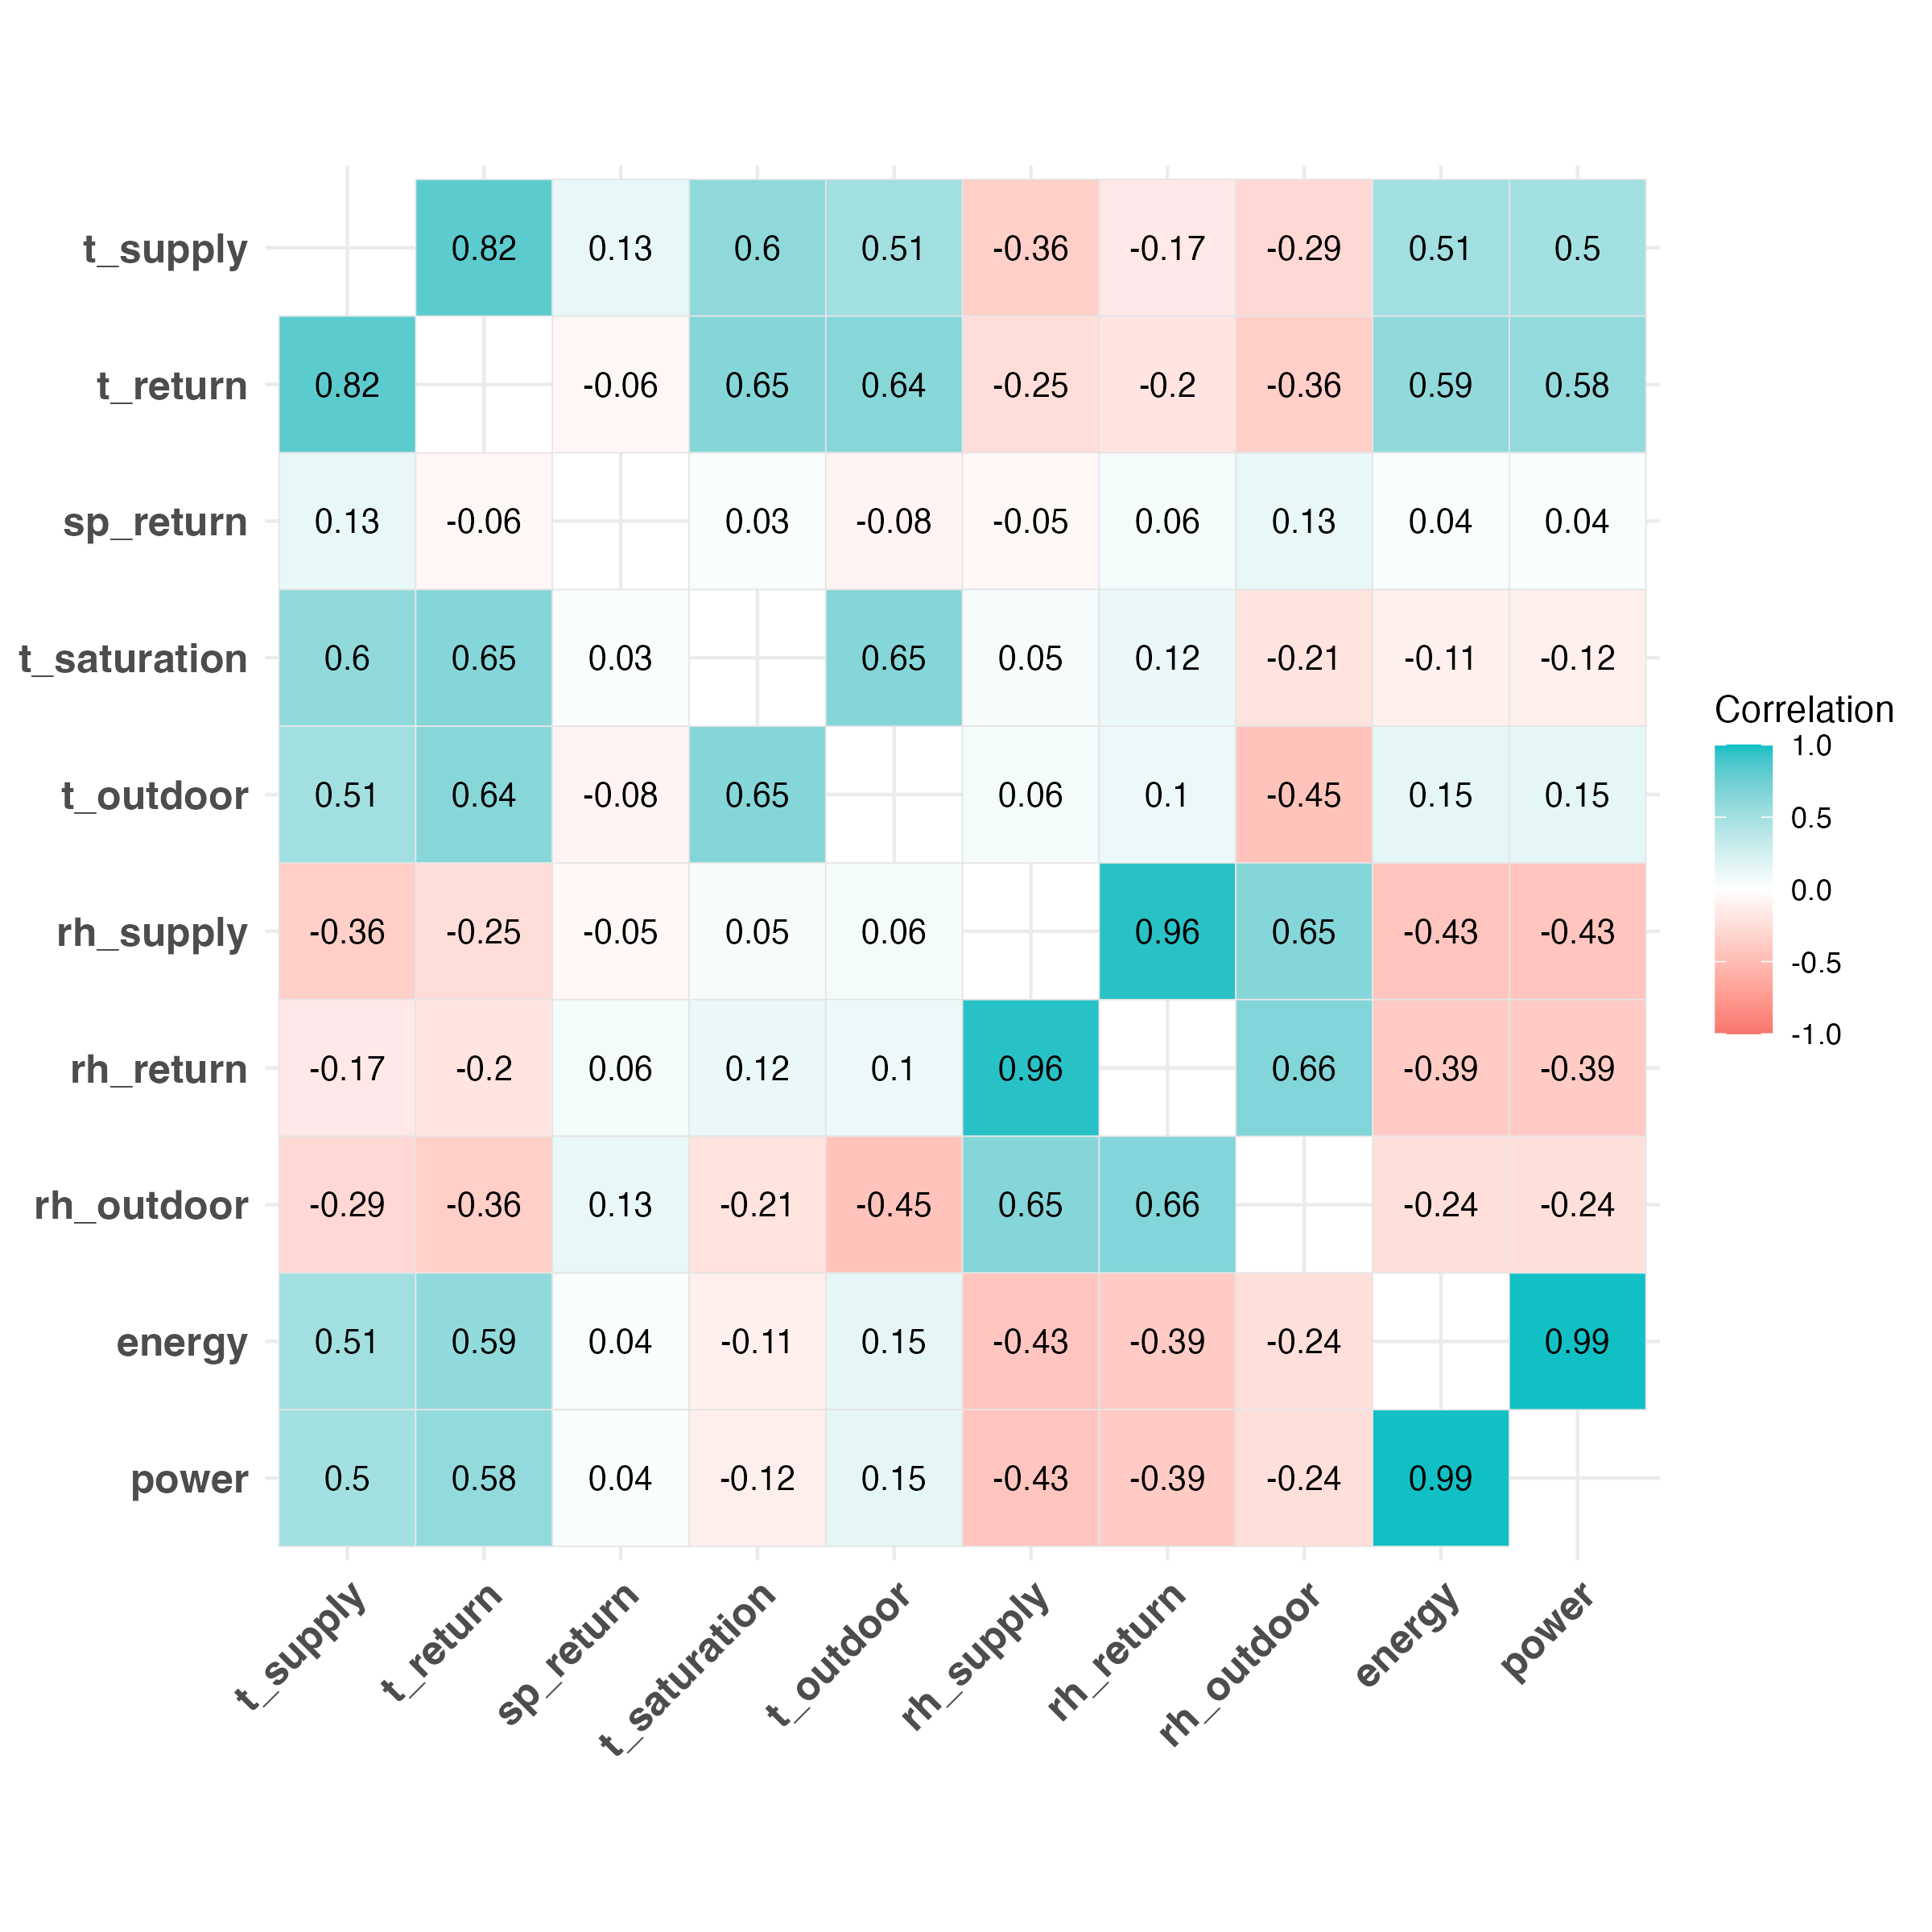
\includegraphics[width=0.8\textwidth]{figures/fig_01_correlation_heatmap.png}
    \caption{Global Pearson correlation heatmap for the Turin HVAC dataset, highlighting high linear correlation across multiple variable pairs.}
    \label{fig:correlation}
\end{figure}

A standard approach to handling high correlation is to reduce the dataset to a subset of minimally correlated variables. However, the Pearson correlation coefficient is an oversimplification that focuses on linear relationships. Visualizing the dataset via a pairwise scatterplot matrix (Figure \ref{fig:scatterplots}) reveals that the actual dependencies between these thermodynamic variables exist regardless of their linear correlation summaries. Instead of simple linear trends, the scatterplots display complex interactions, including distinct data clouds and stacked, parallel bands that correspond to discrete mechanical states.

Attempting to explicitly model these multi-modal dependencies to incorporate causality into a traditional fault-detection model is highly impractical. Manually engineering features to account for these interactions is tedious and it would cause a quadratic increase in the number of variables. 

Instead, \texttt{dynaRchetypes} relies on a multidimensional geometric interpretation of the data. Normal physical operations and machinery dependencies naturally constrain the telemetry, forming dense manifolds---or clouds of points---within the 11-dimensional feature space. When a mechanical fault occurs, this physical causality breaks, causing the resulting telemetry to fall outside these dense regions. The Isolation Forest algorithm is uniquely appropriate for this environment; because it isolates anomalies using random orthogonal hyperplanes rather than traditional distance calculations, it identifies these multidimensional deviations without requiring the user to explicitly uncouple or model the underlying variables. By measuring the average number of random splits required to isolate a point, the algorithm maps shorter path lengths to higher spatial sparsity. This path length is mathematically normalized into a bounded anomaly score between 0 and 1. An anomaly score threshold (e.g., $>0.60$) can then be used to select the most deviating points.

\begin{figure}[htbp]
    \centering
    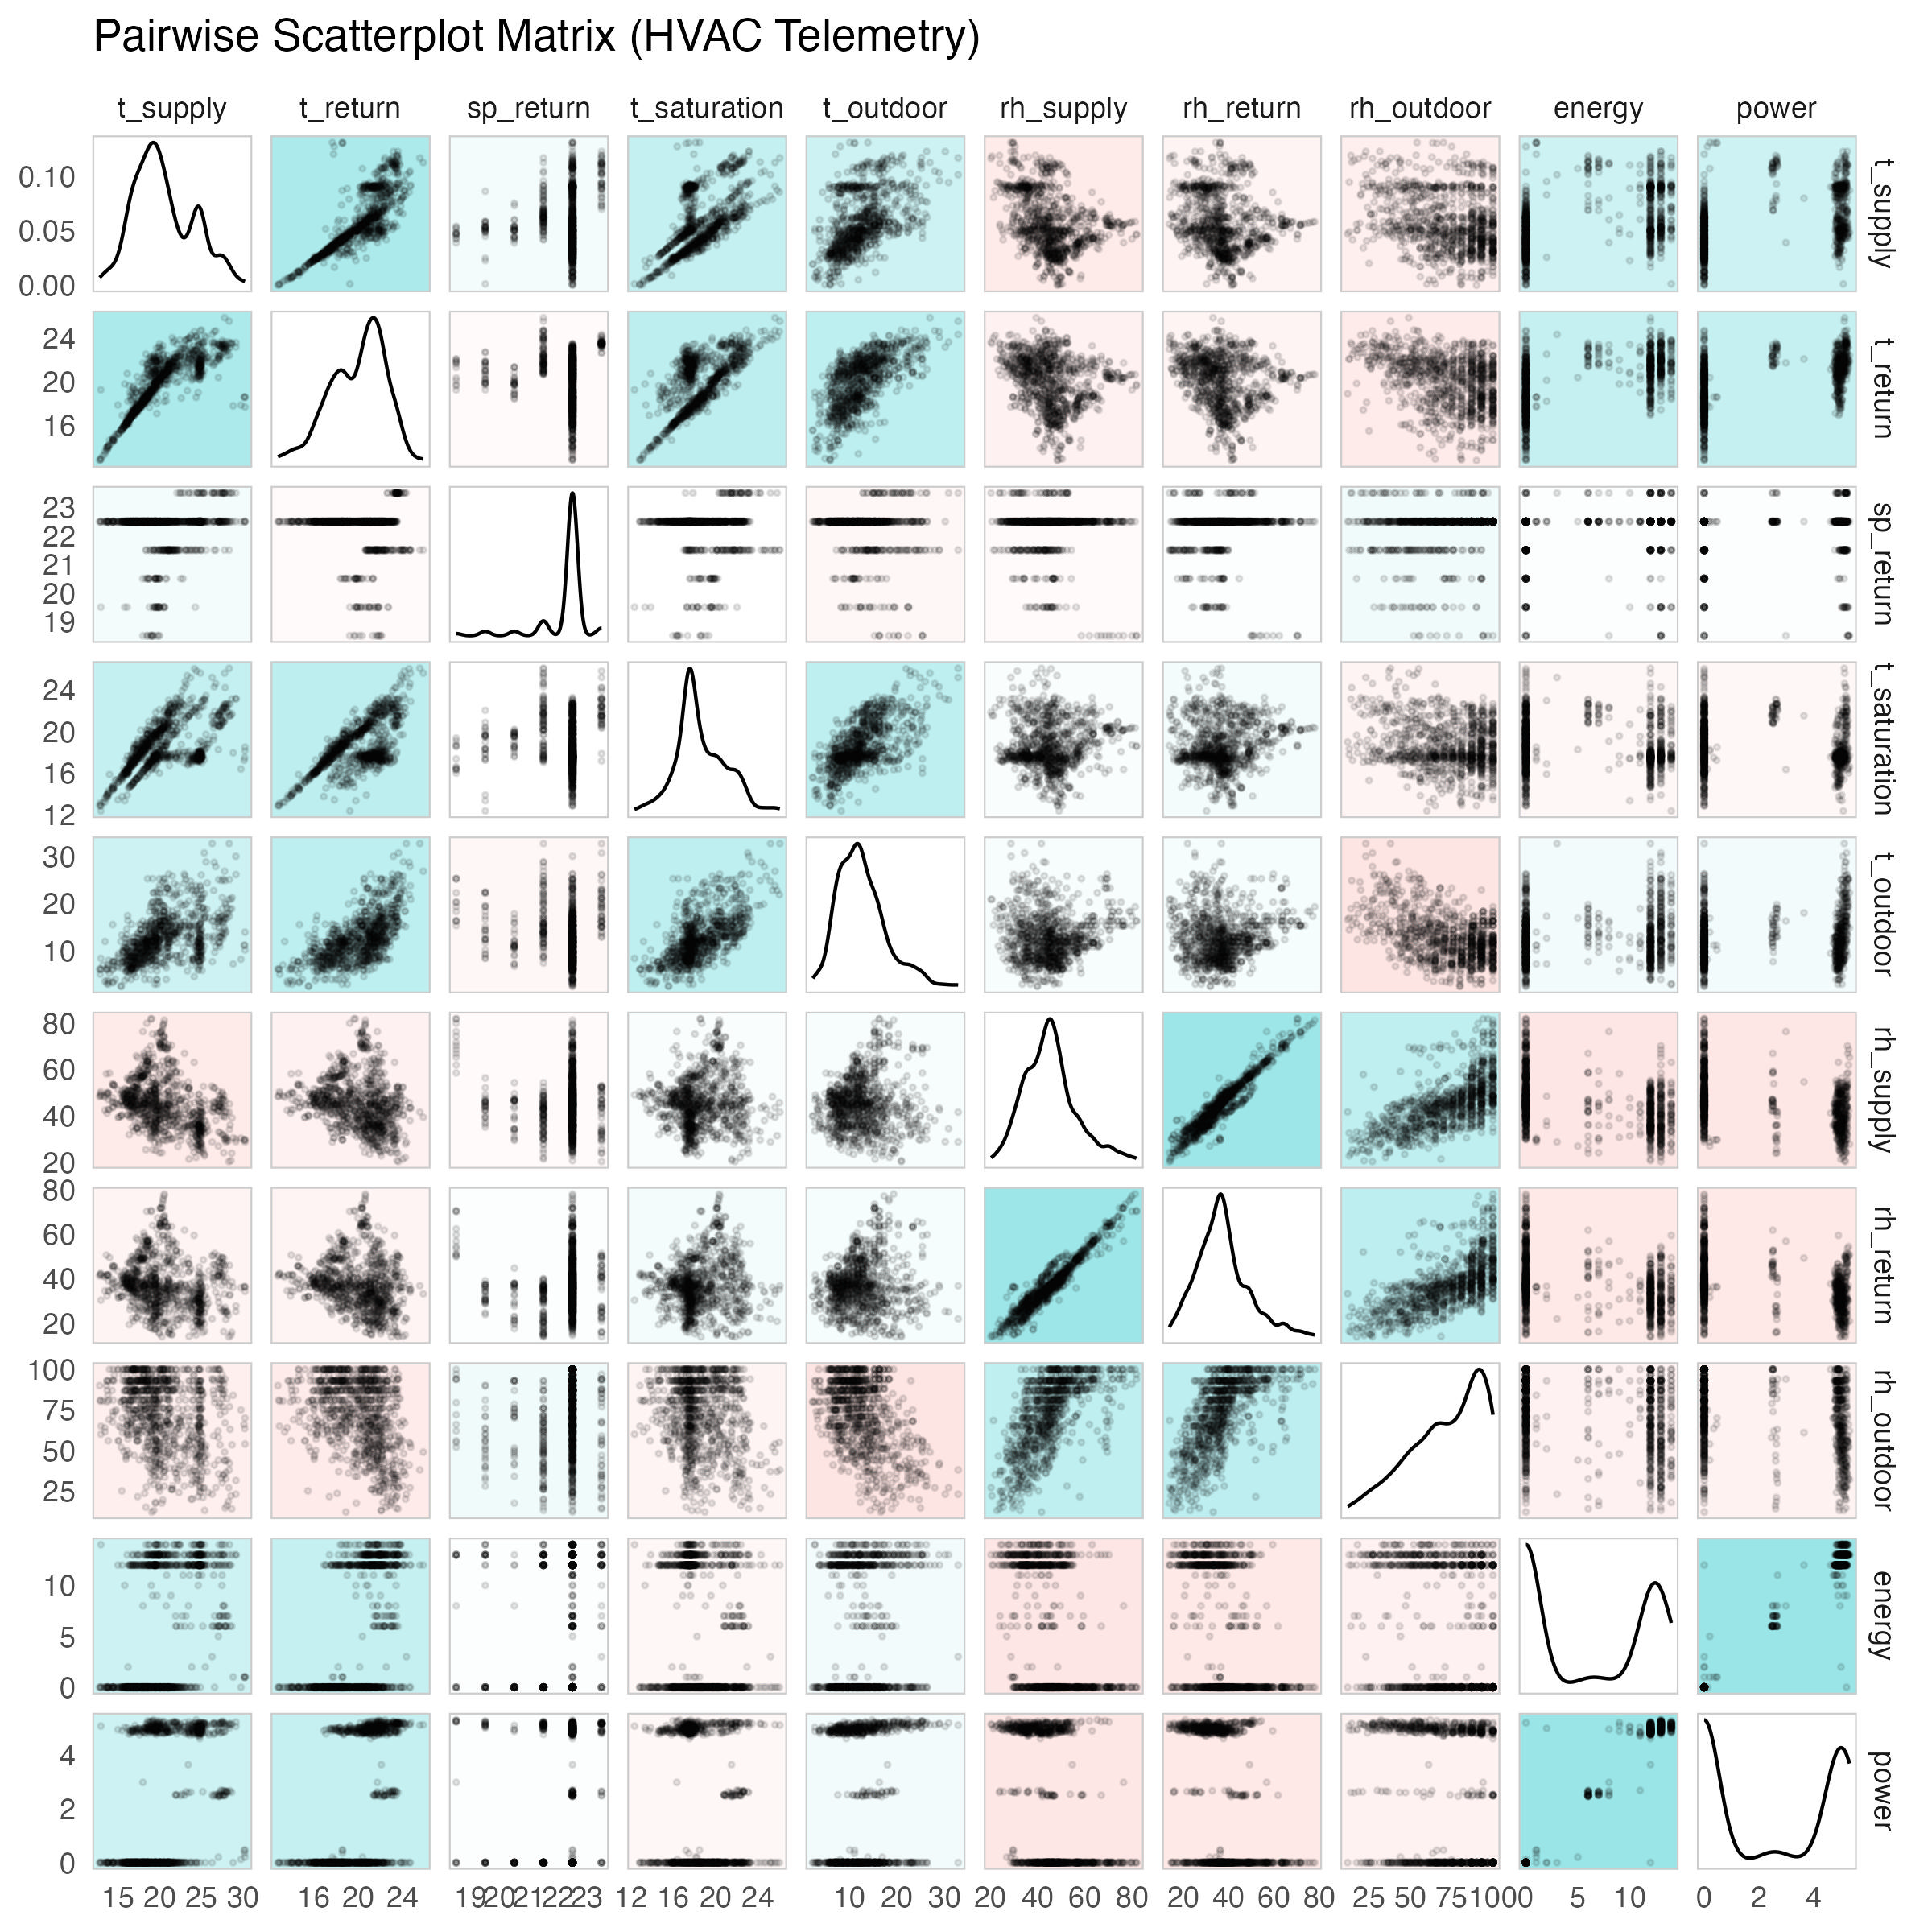
\includegraphics[width=0.8\textwidth]{figures/fig_02_scatterplot_matrix.jpg}
    \caption{Pairwise scatterplot matrix of the HVAC telemetry (sampled at $n=5000$). The plots reveal complex, non-linear operational states and discrete mechanical dependencies that are not captured by linear correlation summaries.}
    \label{fig:scatterplots}
\end{figure}

\section{Illustrative Examples}

\subsection{Baseline Implementation: Unengineered Static Variables}

An intuitive first approach when using \texttt{dynaRchetypes} is to pass the raw dataset (referred to here as \texttt{hvac\_data}) directly into the algorithm without prior feature engineering. In this baseline architecture, the user configures a YAML file (\texttt{naive\_config.yaml}) to list every variable as a \texttt{target\_variable}, leaving the \texttt{context\_variables} empty. The diagnostic pipeline is then executed via standard S4 methods:

\begin{verbatim}
# 1. Initialize engine and ingest unengineered telemetry
engine <- new("DiagnosticEngine", config_path = "naive_config.yaml")
engine <- ingest_telemetry(engine, data = hvac_data)

# 2. Extract anomalies via Isolation Forest
engine <- extract_anomalies(engine, threshold = 0.60)

# 3. Compute MDTW trajectories and calibrate optimal clusters
engine <- compute_distances(engine)
engine <- calibrate(engine, min_k = 2, max_k = 25)
\end{verbatim}

To evaluate the operational viability of fault groupings derived from this raw matrix, we perform an algorithmic threshold sweep. This test maps both the total number of isolated events ($N$) and the resulting optimal number of clusters ($k$) returned by \texttt{calibrate()} across a continuous range of Isolation Forest anomaly thresholds. Internally, the engine determines this optimal $k$ by maximizing the Global Silhouette score, a geometric metric that evaluates cluster structural integrity by measuring how similar an event trajectory is to its own cluster (cohesion) compared to neighboring clusters (separation)\cite{rousseeuw1987silhouettes}. A reliable diagnostic pipeline requires the presence of a "stable region"---a contiguous range of thresholds that yields a consistent optimal $k$.

As shown in Figure \ref{fig:naive_stability}, utilizing raw static variables fails to produce a stable region. The diagnostic pipeline is constrained by two opposing mathematical boundaries. At lower anomaly thresholds (e.g., $<0.59$), the Isolation Forest flags thousands of events, rendering the $O(N^2)$ MDTW distance calculation computationally prohibitive. Conversely, as the threshold increases and the event count ($N$) drops to a manageable size, the optimal number of clusters spikes abruptly, repeatedly hitting the algorithm's maximum evaluation ceiling (\texttt{max\_k} $= 25$ here). 

Scientifically, this spike indicates cluster fragmentation; rather than identifying distinct, repetitive physical fault trajectories, the clustering algorithm is over-segmenting a small number of multidimensional distance calculations into nearly individual singletons ($k \to N$). Furthermore, from an operations research perspective, this behavior is not helpful: a triage system that outputs 25 distinct diagnostics is not practical.

\begin{figure}[htbp]
    \centering
    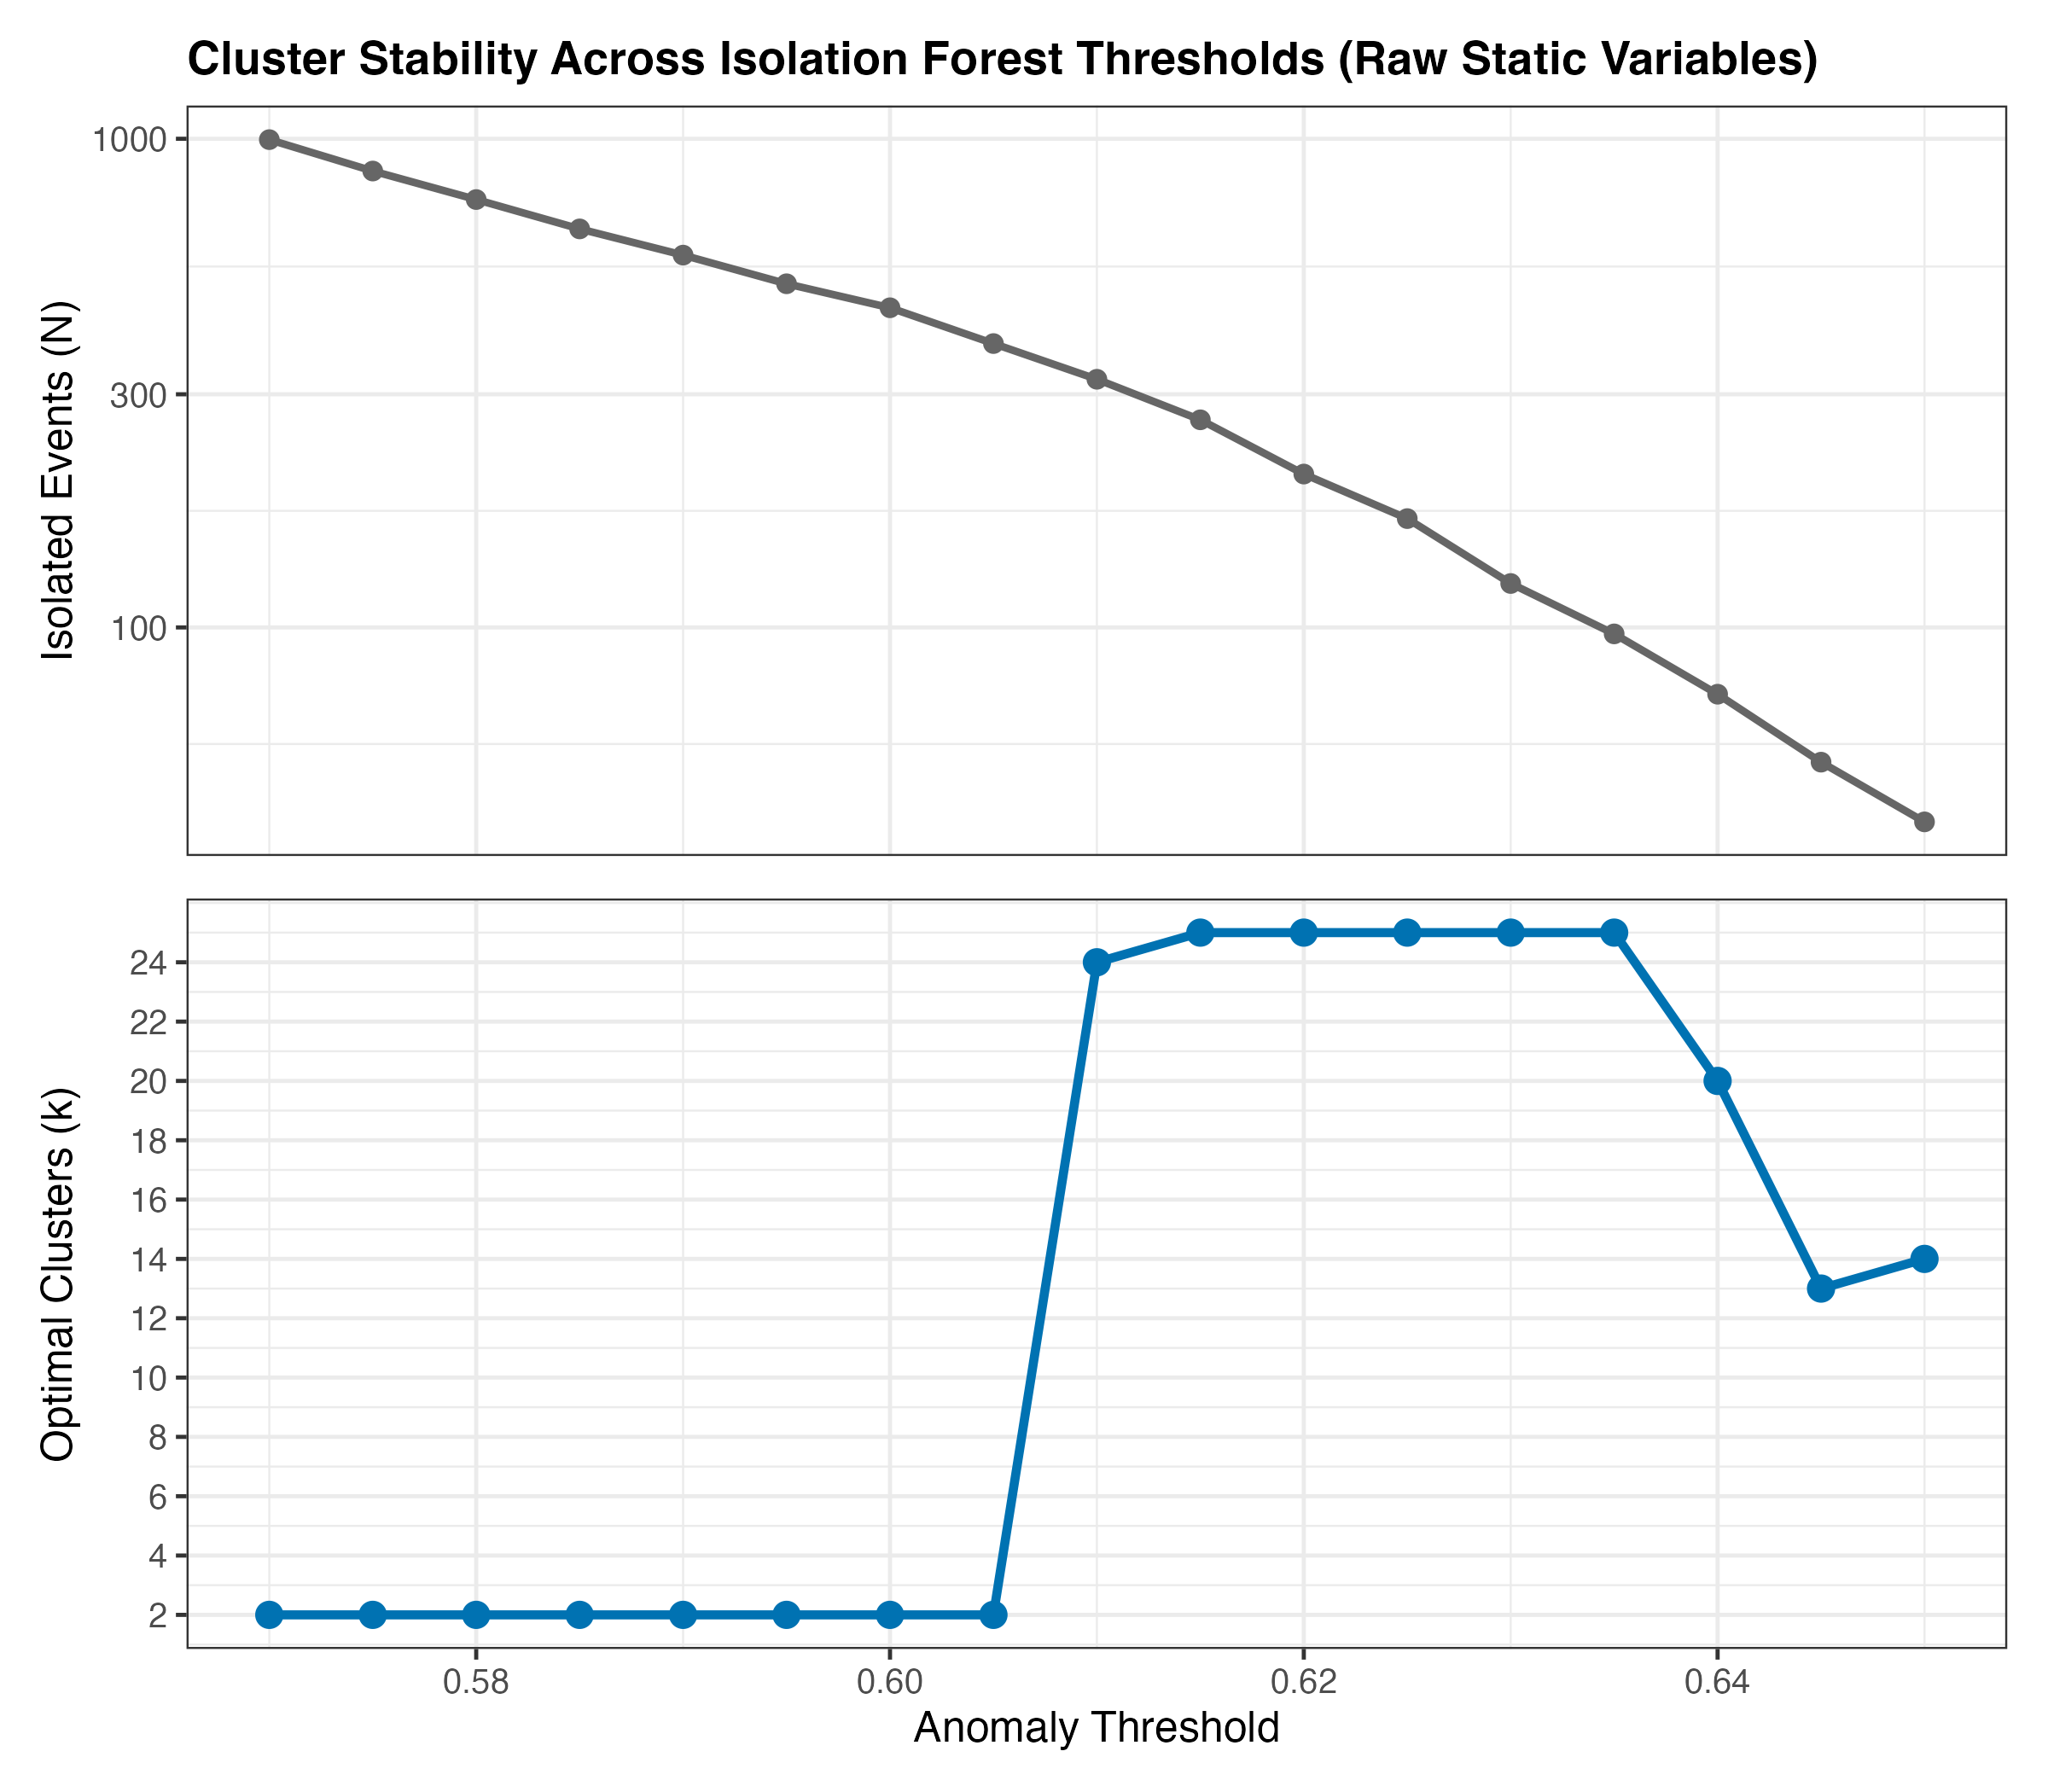
\includegraphics[width=\linewidth]{figures/fig_03_naive_stability.png}
    \caption{Optimal $k$ across an anomaly threshold sweep using the naive architecture (raw, unengineered features). The erratic fluctuation indicates a lack of clustering stability.}
    \label{fig:naive_stability}
\end{figure}

% In HVAC systems, variables often exhibit complex, non-linear dependencies. For example, while the Turin dataset indicates a moderate linear correlation ($r = 0.61$) between supply temperature (\texttt{t\_supply}) and saturation temperature (\texttt{t\_saturation}), a pairwise scatterplot reveals stacked, parallel bands rather than a simple linear trend. These bands represent discrete operational states, such as compressor staging. Attempting to manually engineer features to capture these multi-modal relationships—such as calculating exhaustive pairwise residuals—unnecessarily inflates the feature space. 
% 
% To bypass this problem, \texttt{dynaRchetypes} utilizes an Isolation Forest (IF) for the initial anomaly extraction. Because the IF algorithm partitions data using random orthogonal hyperplanes rather than spatial distance metrics, it is highly robust to these non-linear dependencies. Normal operational data, constrained by physical laws, clusters densely. When a mechanical fault occurs, the telemetry deviates into sparse feature space, where the IF efficiently isolates it. This architecture allows the user to input raw, inherently correlated thermodynamic variables directly into the YAML configuration without requiring explicit mathematical uncoupling.

\subsection{Algorithmic Critique: Mitigating Theoretical Limitations}
While Isolation Forest provides unmatched computational scalability ($O(N \log N)$) and natively handles multi-modal operational states without relying on local density assumptions (unlike DBSCAN or LOF), it possesses two inherent flaws when applied to continuous telemetry:
\begin{itemize}
\item \textbf{Temporal Blindness:} IF is a strictly spatial algorithm. If the chronological rows of a dataset are shuffled, IF returns identical anomaly scores. It has no native concept of sequence or autocorrelation, making it blind to catastrophic instantaneous jumps if the target values remain within globally "normal" bounds.
\item \textbf{Axis-Parallel Bias:} Standard IF draws splits that are strictly horizontal or vertical. When data exhibits strong linear dependencies (such as the diagonal "thermal wedge" between supply and return temperatures), IF builds a jagged "staircase" of cuts. This creates "ghost regions" in the corners of the steps where anomalies can hide undetected.
\end{itemize}

\texttt{dynaRchetypes} mitigates these algorithmic limitations architecturally. The software's YAML schema allows users to define interaction features (e.g., $\Delta T$) that mathematically flatten diagonal dependencies into horizontal planes, eliminating axis-parallel ghost regions. Furthermore, the underlying C++ \texttt{isotree} engine supports Extended Isolation Forests (EIF), which draw cuts at random slopes to naturally slice correlated data. To cure temporal blindness, the architecture mandates kinematic feature engineering prior to spatial evaluation.

\subsection{The Feature Dependency Ablation}
A common assumption in time-series clustering is that trajectory algorithms (like MDTW) can autonomously extract temporal context from raw static inputs. To test this, we conducted a dual ablation study comparing a naive feature matrix (raw temperatures) against a kinetically engineered matrix (temporal derivatives). 

The results mathematically cement the package's design requirement. Euclidean spatial clustering of the raw static variables yielded a near-random Adjusted Rand Index (ARI = 0.226) when compared to MDTW trajectory assignments. However, when kinematic derivatives were injected into the Isolation Forest—effectively smuggling temporal context into the time-blind spatial engine—the ARI jumped to 0.362. This proves that trajectory clustering is inextricably dependent on the upstream anomaly detector extracting kinetically valid structural breaks.

\subsection{Prognostic Architecture: Handling Concept Drift}
Deploying static threshold models in environments subject to seasonal changes inevitably triggers false-positive "alert storms." To validate the prognostic stability of \texttt{dynaRchetypes}, we evaluated the system across a contiguous 5-month block transitioning from Autumn through freezing Winter temperatures. We tested three distinct configurations:

\begin{itemize}
\item \textbf{Engine A (Naive Frozen Baseline):} Trained on 30 days of Autumn raw temperatures. As Winter initiated, the baseline structural trend violently breached the triage threshold, flooding the queue with false positives driven purely by weather.
\item \textbf{Engine B (Kinematic Engine):} Utilizing 15-minute derivatives, this engine maintained a perfectly horizontal, stationary baseline across the 5-month seasonal shift. It successfully isolated acute mechanical snaps while remaining entirely immune to concept drift.
\item \textbf{Engine C (Volatility Engine):} Utilizing 24-hour rolling variance, this engine mapped the slow-creeping degradation of the system's control loops, proving the architecture's capacity for long-term lifecycle monitoring without triggering alert storms.
\end{itemize}

\subsection{Explainable AI and Triage}
Standard machine learning pipelines output abstract multidimensional centroids. To bridge the gap to actionable maintenance, \texttt{dynaRchetypes} leverages algorithmic ablation. By systematically substituting global medians into specific variables and recalculating the Isolation Forest score, the \texttt{explain\_anomaly()} method isolates the "Ablation Drop"—the precise mathematical contribution of a specific sensor to the structural break. This translates abstract geometric sparsity directly into a physical work order (e.g., "Fault driven by a sudden 45\% drop in Expected Power").

\section{Impact and Best Practices}
The primary impact of \texttt{dynaRchetypes} lies in bridging the historical gap between abstract multidimensional machine learning and actionable facility management, achieving robust clustering without the need for labeled training data. 

To achieve successful operational deployment, users must acknowledge the following best practices identified during the package's development:
\begin{itemize}
\item \textbf{Kinematic Requirement:} Raw, static variables are insufficient for trajectory clustering. Users must engineer temporal derivatives to provide the upstream Isolation Forest with thermodynamic context.
\item \textbf{Curse of Dimensionality Avoidance:} Instead of exploding the feature matrix with dozens of pairwise residuals to map nonlinear transfer functions, users should rely on the Isolation Forest's native topological sparsity detection to identify broken causal dependencies.
\item \textbf{Hyperparameter Stability:} Users must utilize the included \texttt{evaluate\_forest\_stability()} helper to prove that their selected tree count ($ntrees$) achieves convergence (e.g., Spearman $\rho > 0.95$), preventing triage queues from being dictated by stochastic model variance.
\end{itemize}

\section{Conclusions}

\texttt{dynaRchetypes} provides a highly structured, parameter-driven S4 architecture for extracting and clustering multidimensional telemetry faults. By synthesizing Isolation Forests with MDTW and implementing built-in XAI and prognostic drift validations, the software successfully translates noisy sensor data into a concise, stable set of operational dispatch queues. The software’s strict separation of mathematical targets from interpretable context ensures that the final outputs are not just mathematically sound, but immediately actionable for operators.

\bibliographystyle{elsarticle-num}
\bibliography{references}

\end{document}